\begin{frame}{Segment-Level Recurrence}
  \begin{columns}[T,onlytextwidth]
    \column{0.46\textwidth}
      \begin{itemize}\footnotesize\itemsep0.4em
        \item[\textcolor{red}{$\blacktriangleright$}] Split $n$ tokens into segments of $s$ tokens and process them in order, carrying a memory of $M$ vectors from one segment to the next. Attention then costs about $n\,(s+M)$ instead of $n^2$.
        \item[\textcolor{red}{$\blacktriangleright$}] \textbf{Cached states.} Layer $\ell$ of segment $\tau$ also attends to the layer-$(\ell-1)$ states that segment $\tau-1$ left behind. A \textbf{stop-gradient} makes this cache a constant in the backward pass, so no gradient enters the previous segment.
        \item[\textcolor{red}{$\blacktriangleright$}] \textbf{Reach.} Each layer looks one segment further back, so $L$ layers reach about $L\cdot s$ tokens.
        \item[\textcolor{red}{$\blacktriangleright$}] Sliding-window attention with window $w$ also reaches $L\cdot w$ through depth, but runs over the whole sequence in one pass. Here only one segment and its cache are held at a time.
      \end{itemize}
    \column{0.52\textwidth}
      \centering
      \vspace{0.2em}
      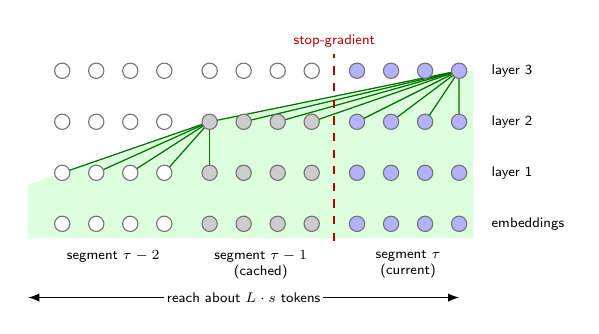
\begin{tikzpicture}[font=\sffamily\scriptsize, >=latex, scale=0.72,
          every node/.style={transform shape},
          tok/.style={circle, draw=black!55, minimum size=0.27cm, inner sep=0pt},
          curtok/.style={tok, fill=blue!30},
          memtok/.style={tok, fill=gray!40},
          oldtok/.style={tok, fill=white},
          att/.style={green!45!black, line width=0.45pt}]
        \fill[green!13] (7.0,2.7) -- (2.6,1.8) -- (0,0.9) -- (-0.6,0.69) -- (-0.6,-0.25) -- (7.25,-0.25) -- (7.25,2.7) -- cycle;
        % Edges run centre to centre and are drawn before the nodes, so the nodes hide their ends.
        \foreach \t in {0,1,2,3} {
          \draw[att] (7.0,2.7) -- ({2.6+0.6*\t},1.8);
          \draw[att] (7.0,2.7) -- ({5.2+0.6*\t},1.8);
          \draw[att] (2.6,1.8) -- ({0.6*\t},0.9);
        }
        \draw[att] (2.6,1.8) -- (2.6,0.9);
        \foreach \l in {0,1,2,3} {
          \foreach \t in {0,1,2,3} {
            \node[oldtok] at ({0.6*\t},{0.9*\l}) {};
            \node[curtok] at ({5.2+0.6*\t},{0.9*\l}) {};
          }
        }
        % The top layer of segment tau-1 is never read by segment tau, so it is not part of the cache.
        \foreach \l in {0,1,2} {
          \foreach \t in {0,1,2,3} {
            \node[memtok] at ({2.6+0.6*\t},{0.9*\l}) {};
          }
        }
        \foreach \t in {0,1,2,3} {
          \node[oldtok] at ({2.6+0.6*\t},2.7) {};
        }
        \draw[red!70!black, dashed, thick] (4.8,-0.3) -- (4.8,3.0);
        \node[red!70!black, anchor=south] at (4.8,3.0) {stop-gradient};
        \node[align=center, anchor=north] at (0.9,-0.35) {segment $\tau-2$};
        \node[align=center, anchor=north] at (3.5,-0.35) {segment $\tau-1$\\(cached)};
        \node[align=center, anchor=north] at (6.1,-0.35) {segment $\tau$\\(current)};
        \node[anchor=west] at (7.45,0) {embeddings};
        \node[anchor=west] at (7.45,0.9) {layer 1};
        \node[anchor=west] at (7.45,1.8) {layer 2};
        \node[anchor=west] at (7.45,2.7) {layer 3};
        \draw[<->] (-0.6,-1.3) -- (7.0,-1.3) node[midway, fill=white, inner sep=1.5pt] {reach about $L\cdot s$ tokens};
      \end{tikzpicture}\\[0.4em]
      {\scriptsize Here $s=4$ and $L=3$. The top state of the last token in segment $\tau$ reads layer 2 of segments $\tau-1$ and $\tau$; the cached state it reaches in segment $\tau-1$ had read layer 1 of segment $\tau-2$. Shaded: everything that state can depend on.\par}
  \end{columns}
\end{frame}

\begin{frame}{Transformer-XL: Reusing the Previous Segment}
  \begin{itemize}\footnotesize\itemsep0.3em
    \item[\textcolor{red}{$\blacktriangleright$}] Transformer-XL (Dai et al., ACL 2019) feeds every layer the cached states of the previous segment:
      \[ \tilde{H}^{\ell-1}_{\tau} = \big[\,\mathrm{SG}(H^{\ell-1}_{\tau-1}) \circ H^{\ell-1}_{\tau}\,\big], \qquad H^{\ell}_{\tau} = \mathrm{Layer}\big(H^{\ell-1}_{\tau} W_q,\; \tilde{H}^{\ell-1}_{\tau} W_k,\; \tilde{H}^{\ell-1}_{\tau} W_v\big). \]
      $H^{\ell}_{\tau} \in \mathbb{R}^{s \times d}$ holds the layer-$\ell$ states of segment $\tau$ ($d$: model width; $H^{0}$: token embeddings). $\mathrm{SG}$ is the stop-gradient and $\circ$ concatenates along the sequence, so the $s$ queries of the segment meet $2s$ keys and values. $W_q, W_k, W_v$ are the layer's projections; $\mathrm{Layer}$ is causal attention plus the feed-forward block. The cache can hold $M$ states over several segments: $M=s$ in training, longer at evaluation.
    \item[\textcolor{red}{$\blacktriangleright$}] \textbf{Evaluation.} A fixed-window model recomputes a whole window for every predicted token. Reusing the cache is up to \textbf{1,874$\times$} faster per token on enwik8 at an attention length of 3,800.
  \end{itemize}
  \centering
  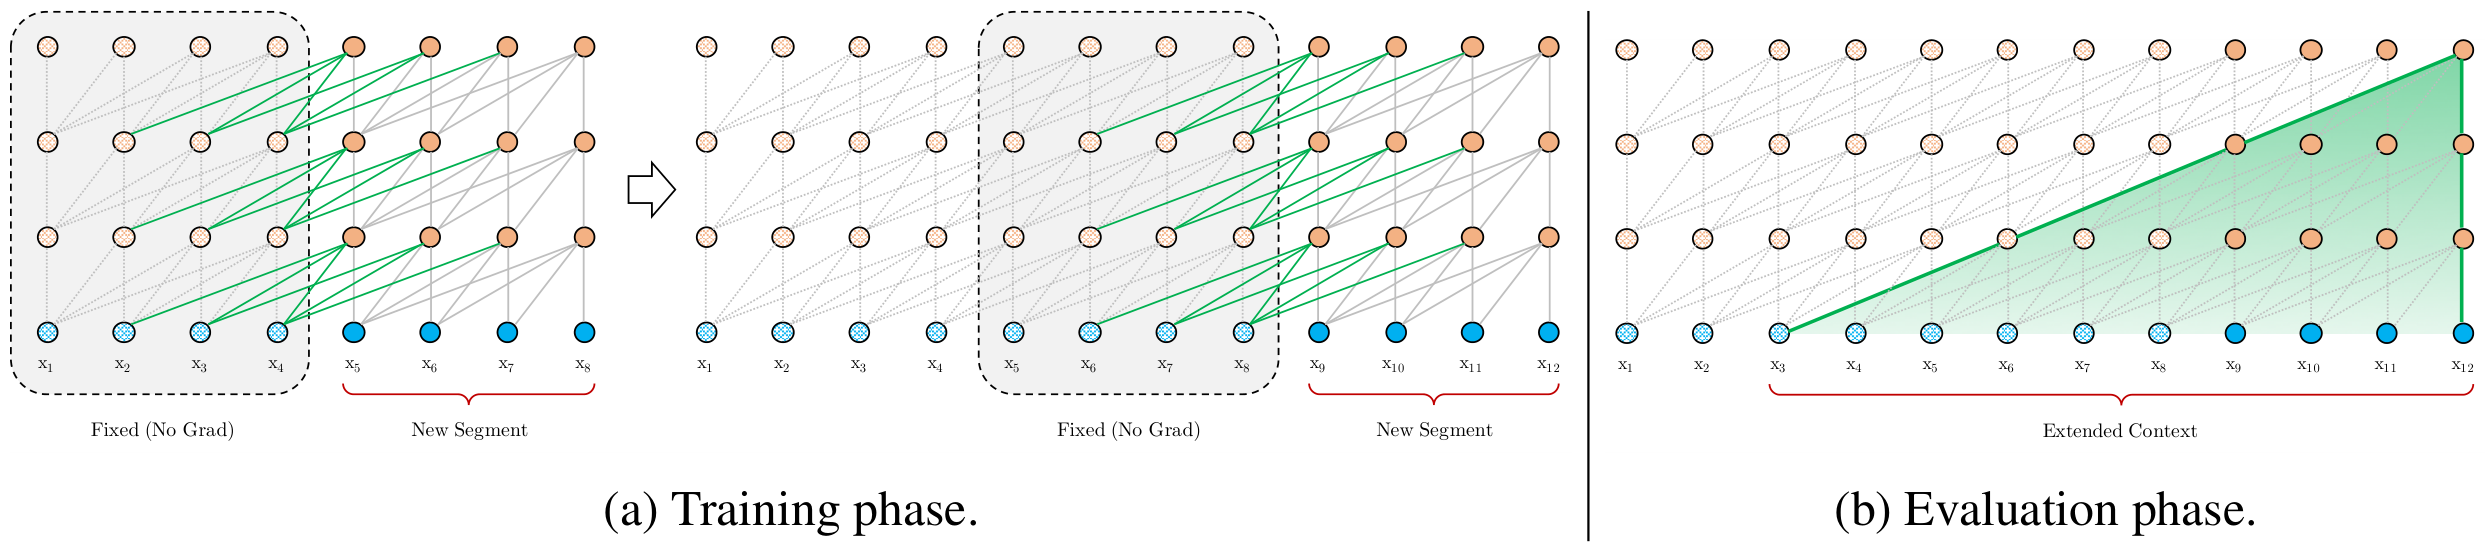
\includegraphics[width=\textwidth,height=0.33\textheight,keepaspectratio]{images/long-context/transformerxl_fig2_training_and_evaluation.png}\\[0.2em]
  {\scriptsize Dai et al., ``Transformer-XL: Attentive Language Models Beyond a Fixed-Length Context,'' ACL 2019, \href{https://arxiv.org/abs/1901.02860v3}{arXiv:1901.02860v3}, Figure~2.\par}
\end{frame}

\begin{frame}{Transformer-XL: Relative Positions}
  \begin{columns}[T,onlytextwidth]
    \column{0.58\textwidth}
      \begin{itemize}\footnotesize\itemsep0.35em
        \item[\textcolor{red}{$\blacktriangleright$}] \textbf{Absolute positions break.} Every segment reuses positions $1,\dots,s$, so token $j$ of segment $\tau$ and token $j$ of segment $\tau+1$ get the same position vector, and the model cannot tell which came first.
        \item[\textcolor{red}{$\blacktriangleright$}] \textbf{Fix:} put the distance $i-j$ into every attention score, as RoPE and ALiBi also do. For query $i$ and key $j$:
          \[ A_{i,j} = \underbrace{q_i^{\top} k_j}_{(a)} + \underbrace{q_i^{\top} W_{k,R}\, r_{i-j}}_{(b)} + \underbrace{u^{\top} k_j}_{(c)} + \underbrace{v^{\top} W_{k,R}\, r_{i-j}}_{(d)} \]
          (a) content addressing, (b) a position term that depends on the query's content, (c) a global content bias, (d) a global position bias. $q_i$ and $k_j$ come from content alone, $r_{i-j}$ is a fixed sinusoidal encoding of the distance, $W_{k,R}$ is its key projection, and $u, v \in \mathbb{R}^{d}$ are learned vectors shared by all query positions.
        \item[\textcolor{red}{$\blacktriangleright$}] Fixed sinusoids let a model trained with a short memory use a longer one: on WikiText-103, 384 tokens of attention in training and 1,600 at evaluation.
      \end{itemize}
    \column{0.40\textwidth}
      \centering
      {\scriptsize
      \begin{tabular}{l r}
        \toprule
        \textbf{Model (WikiText-103)} & \textbf{RECL} \\
        \midrule
        Transformer-XL, 151M & 900 \\
        QRNN & 500 \\
        LSTM & 400 \\
        \midrule
        Transformer-XL, 128M & 700 \\
        \quad without recurrence & 300 \\
        Vanilla Transformer & 128 \\
        \bottomrule
      \end{tabular}\par}
      \vspace{0.5em}
      \begin{itemize}\scriptsize\itemsep0.25em
        \item[\textcolor{red}{$\blacktriangleright$}] \textbf{RECL} (relative effective context length, in words): grow the context until extra words cut perplexity by less than 1\%, measured against the best model of the same group on the 10\% hardest tokens. QRNN is a quasi-recurrent network.
        \item[\textcolor{red}{$\blacktriangleright$}] Hence the headline: 80\% longer than RNNs and 450\% longer than a vanilla Transformer.
        \item[\textcolor{red}{$\blacktriangleright$}] At publication: perplexity 18.3 on WikiText-103 (previous best 20.5) and 0.99 bits per character on enwik8.
      \end{itemize}
  \end{columns}
  \vspace{0.1em}
  {\scriptsize Dai et al., \href{https://arxiv.org/abs/1901.02860v3}{arXiv:1901.02860v3}, Section~3.3, Tables~1, 2 and 8, Appendix~C.}
\end{frame}

\begin{frame}{Compressive Transformer and PG-19}
  \begin{columns}[T,onlytextwidth]
    \column{0.52\textwidth}
      \begin{itemize}\footnotesize\itemsep0.3em
        \item[\textcolor{red}{$\blacktriangleright$}] Each layer keeps two first-in, first-out memories: the last $M$ states, as in Transformer-XL, and $M_c$ compressed states. The $s$ states evicted by each new segment go through a compression function $f_c$ that returns $s/c$ compressed states ($c$: compression rate).
        \item[\textcolor{red}{$\blacktriangleright$}] Attention reads compressed memory, memory and segment together, so $L$ layers reach $L\,(s+M+c\,M_c)$ tokens.
        \item[\textcolor{red}{$\blacktriangleright$}] $f_c$ tried: pooling or 1D convolution with kernel and stride $c$, dilated convolution, or keeping the most-attended memories.
        \item[\textcolor{red}{$\blacktriangleright$}] $f_c$ is trained locally, without backpropagation through time (BPTT) over long unrolls, by an \textbf{attention-reconstruction} loss:
          \[ \mathcal{L}_{\mathrm{attn}} = \big\lVert \mathrm{attn}(h, m) - \mathrm{attn}\big(h, f_c(m)\big) \big\rVert_2 \]
          $h$: the segment's states; $m$: the evicted memories; $\mathrm{attn}$: the layer's content-only attention, frozen. What nothing attends to may be dropped. Best on Enwik8: a convolution with this loss, 0.973 bits per character (0.984 with an auto-encoding loss).
      \end{itemize}
    \column{0.46\textwidth}
      \centering
      \vspace{0.3em}
      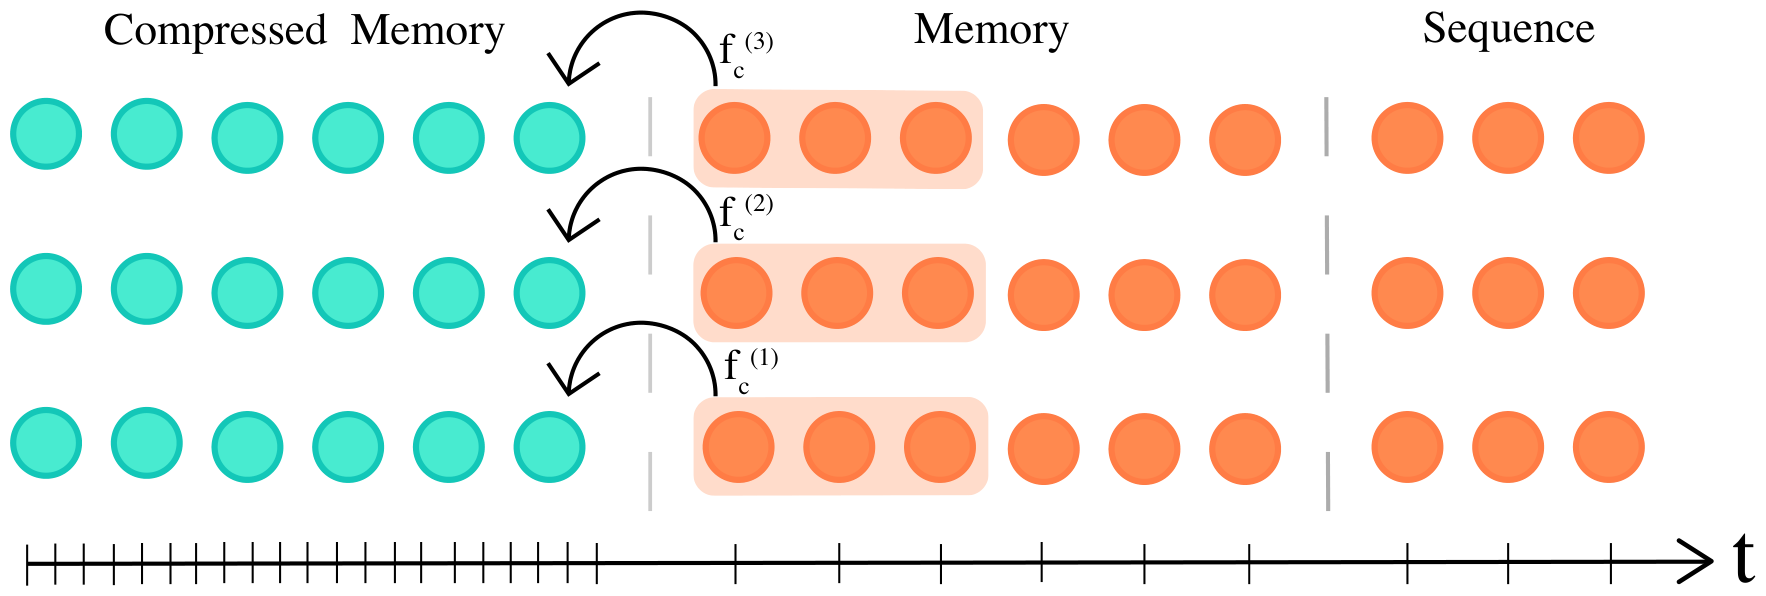
\includegraphics[width=\linewidth,height=0.30\textheight,keepaspectratio]{images/long-context/compressive_fig1_memory_and_compressed_memory.png}\\[0.2em]
      {\scriptsize Three layers, $s=3$, $M=M_c=6$, $c=3$. Rae et al., ``Compressive Transformers for Long-Range Sequence Modelling,'' ICLR 2020, \href{https://openreview.net/forum?id=SylKikSYDH}{openreview.net/forum?id=SylKikSYDH}, Figure~1.\par}
      \vspace{0.6em}
      \begin{itemize}\footnotesize\itemsep0.3em
        \item[\textcolor{red}{$\blacktriangleright$}] \textbf{PG-19}, released with the model: 28,752 Project Gutenberg books published before 1919, 11\,GB of text, 69K words per book on average against 3.6K for a WikiText-103 article.
        \item[\textcolor{red}{$\blacktriangleright$}] Test perplexity with 36 layers: 33.6 for the Compressive Transformer, 36.3 for Transformer-XL.
      \end{itemize}
  \end{columns}
\end{frame}

\begin{frame}{Memorizing Transformers: kNN over Past Keys}
  \begin{columns}[T,onlytextwidth]
    \column{0.56\textwidth}
      \begin{itemize}\footnotesize\itemsep0.3em
        \item[\textcolor{red}{$\blacktriangleright$}] Layer 9 of 12 is \textbf{kNN-augmented}. After each 512-token training step, its (key, value) pairs join an external memory that keeps the latest $M$ pairs per head (up to 262K) and is emptied at each new document.
        \item[\textcolor{red}{$\blacktriangleright$}] Each query fetches its top $k=32$ keys by approximate $k$-nearest-neighbour (kNN) search, as RAG retrievers do; about 90\% of the true top $k$ come back. A learned gate per head mixes the two results:
          \[ g = \sigma(b_g), \qquad V_a = g \odot V_m + (1-g) \odot V_c \]
          $V_a$: the combined attention output; $V_m$: attention over the retrieved pairs; $V_c$: local attention; $b_g$: a learned scalar per head; $\sigma$: the sigmoid.
        \item[\textcolor{red}{$\blacktriangleright$}] \textbf{No gradient into the memory}, so stored pairs are reused across steps and $M$ can grow. Old keys go stale as the weights change; normalizing keys and queries at least keeps old and new keys at the same magnitude.
        \item[\textcolor{red}{$\blacktriangleright$}] C4 web documents over 4K tokens: perplexity 17.20 without memory, 14.42 with an 8K memory. On arXiv math, an 8K memory matched a vanilla Transformer with 5$\times$ the parameters.
      \end{itemize}
    \column{0.42\textwidth}
      \centering
      \vspace{0.4em}
      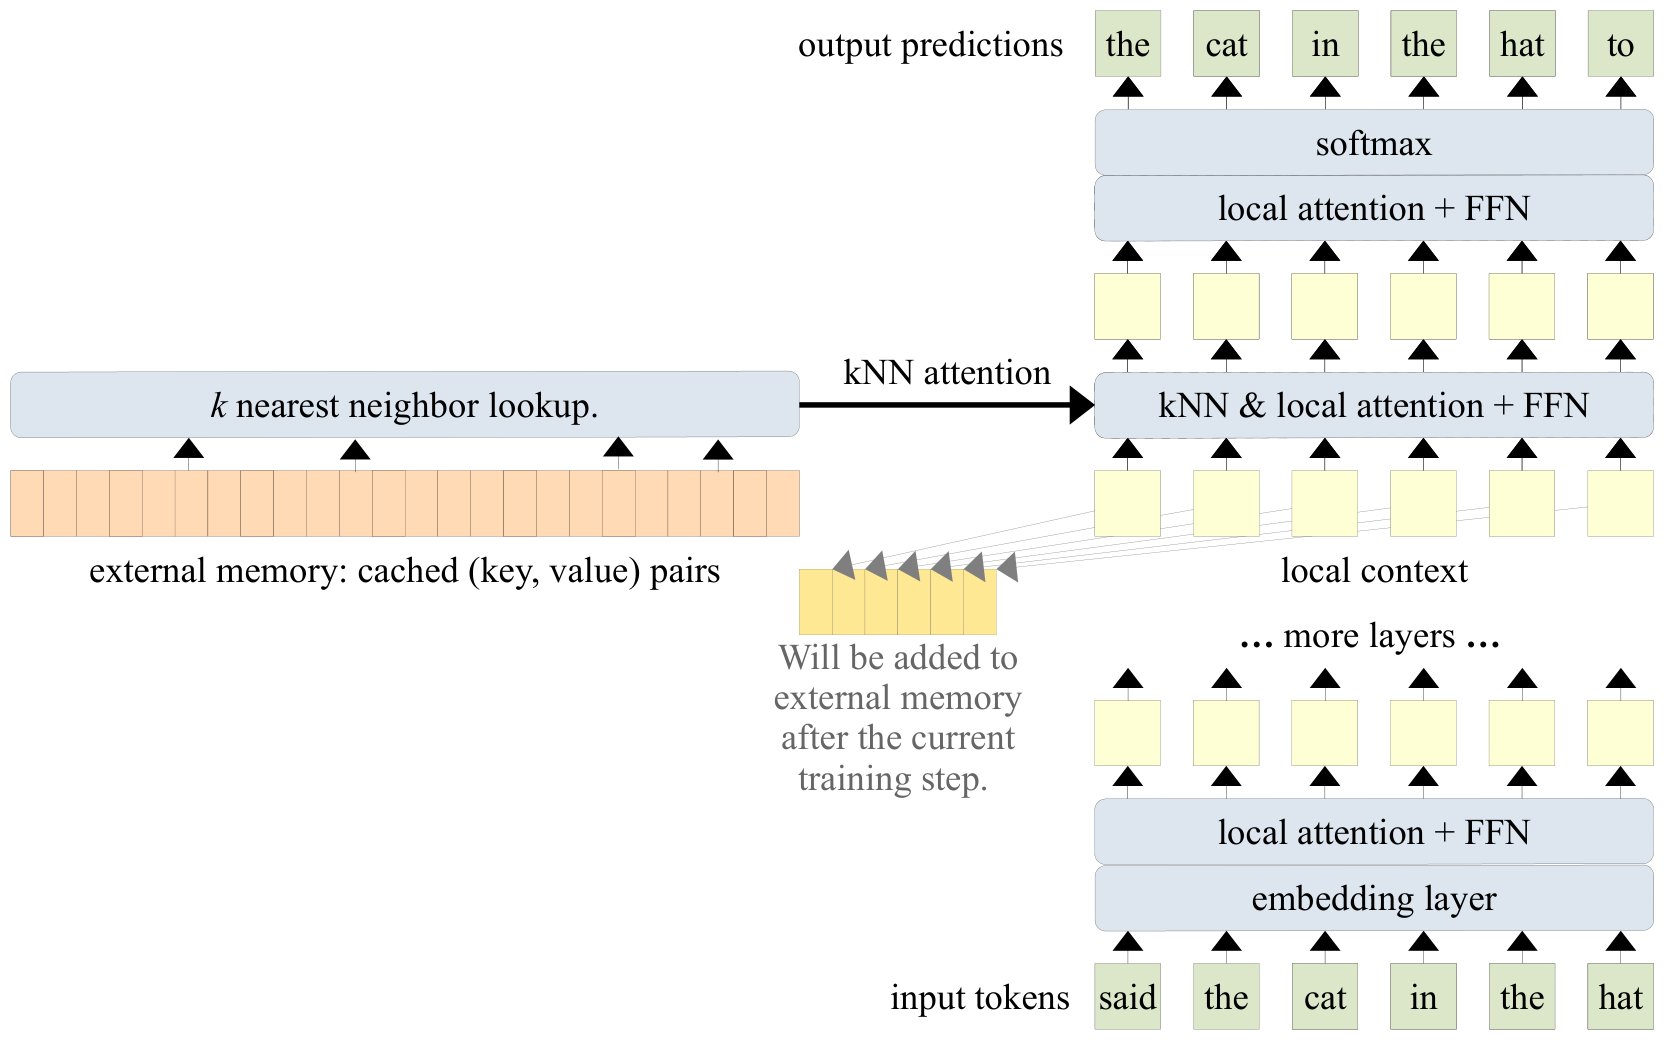
\includegraphics[width=\linewidth,height=0.62\textheight,keepaspectratio]{images/long-context/memorizing_fig2_knn_augmented_layer.png}\\[0.2em]
      {\scriptsize Wu et al., ``Memorizing Transformers,'' ICLR 2022, \href{https://arxiv.org/abs/2203.08913v1}{arXiv:2203.08913v1}, Figure~2.\par}
  \end{columns}
\end{frame}

\begin{frame}{Recurrent Memory Transformer (RMT)}
  \begin{columns}[T,onlytextwidth]
    \column{0.52\textwidth}
      \begin{itemize}\footnotesize\itemsep0.3em
        \item[\textcolor{red}{$\blacktriangleright$}] $M$ memory tokens (real-valued vectors) go at both ends of every segment; $X_\tau$ holds the embeddings of its $s$ tokens:
          \[ \begin{aligned}
            \tilde{X}_\tau &= [\,H^{\mathrm{mem}}_\tau \circ X_\tau \circ H^{\mathrm{mem}}_\tau\,] \\
            [\,H^{\mathrm{read}}_\tau \circ H_\tau \circ H^{\mathrm{write}}_\tau\,] &= \mathrm{Transformer}(\tilde{X}_\tau) \\
            H^{\mathrm{mem}}_{\tau+1} &= H^{\mathrm{write}}_\tau
          \end{aligned} \]
          $H_\tau$: the segment's outputs. Under the causal mask the segment reads the start copy; the end copy sees the whole segment and becomes the next memory.
        \item[\textcolor{red}{$\blacktriangleright$}] The Transformer is unchanged: memory exists only in its input and output.
        \item[\textcolor{red}{$\blacktriangleright$}] Trained with BPTT over 0 to 4 previous segments: gradients reach earlier segments through the memory.
        \item[\textcolor{red}{$\blacktriangleright$}] WikiText-103, 150-token segments: 10 and 25 memory tokens give perplexity 25.04 and 24.85, close to 24.68 for Transformer-XL with 75 cached states per layer.
      \end{itemize}
    \column{0.46\textwidth}
      \centering
      \vspace{0.3em}
      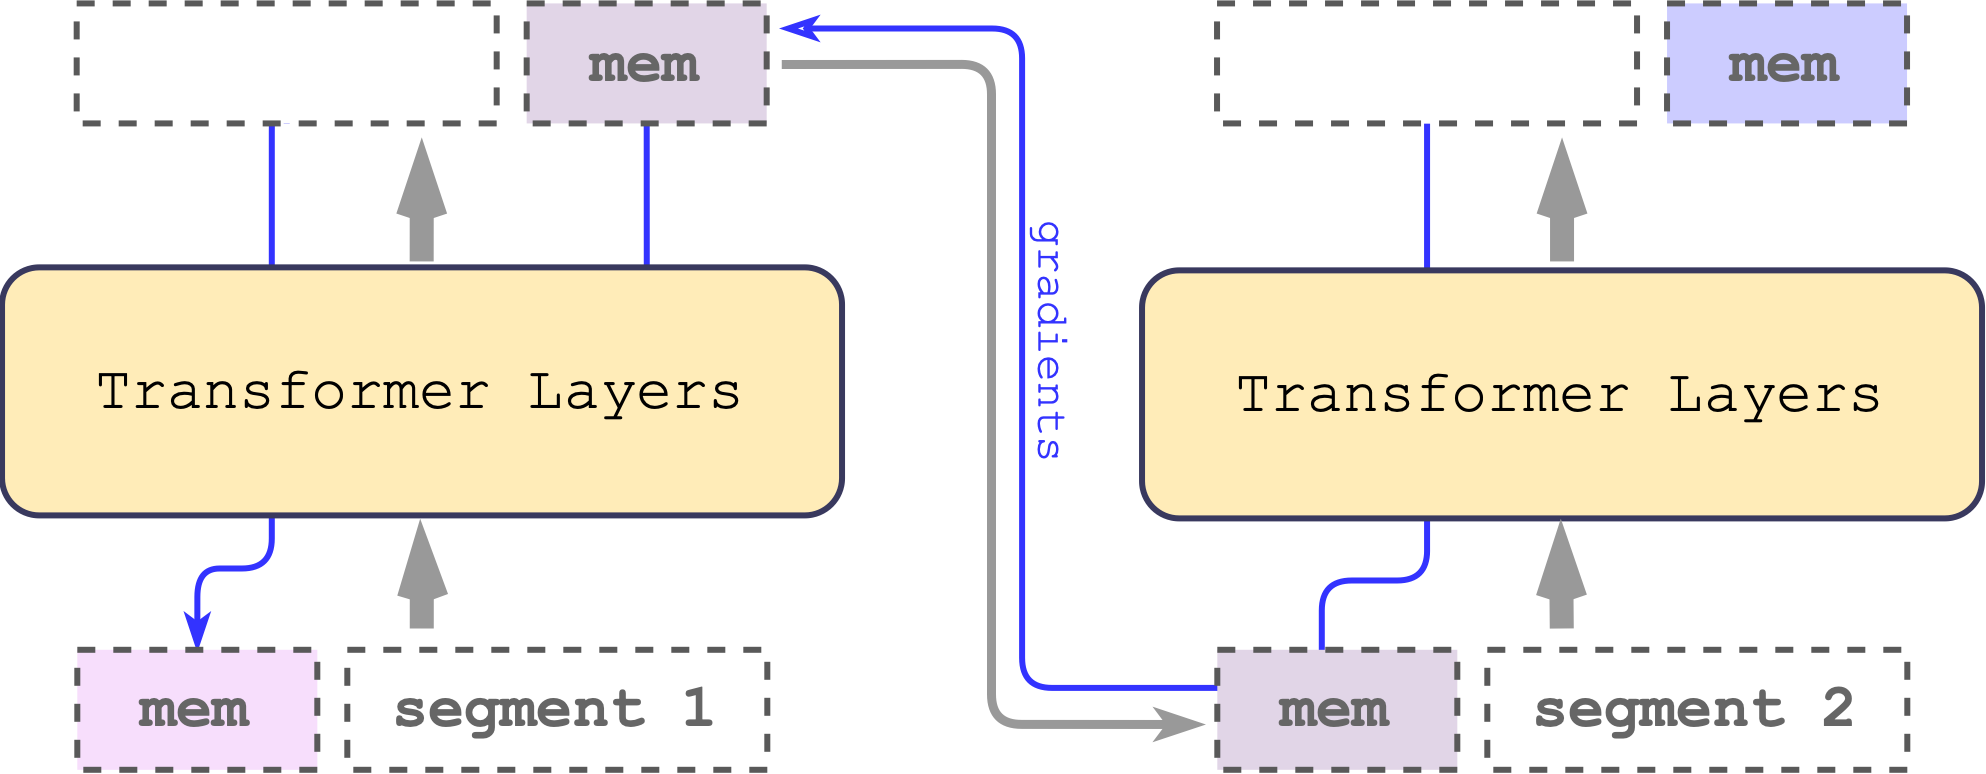
\includegraphics[width=\linewidth,height=0.28\textheight,keepaspectratio]{images/long-context/rmt_fig1_memory_tokens_between_segments.png}\\[0.2em]
      {\scriptsize Bulatov, Kuratov \& Burtsev, ``Recurrent Memory Transformer,'' NeurIPS 2022, \href{https://arxiv.org/abs/2207.06881v2}{arXiv:2207.06881v2}, Figure~1.\par}
      \vspace{0.7em}
      {\scriptsize
      \begin{tabular}{@{}>{\raggedright\arraybackslash}p{1.25cm} >{\raggedright\arraybackslash}p{2.2cm} >{\raggedright\arraybackslash}p{2.0cm}@{}}
        \toprule
         & \textbf{Transformer-XL} & \textbf{RMT} \\
        \midrule
        Carried & $M$ states per layer, $M\cdot L$ in all & $M$ vectors \\
        \addlinespace[0.15em]
        Gradient & stopped at the segment & BPTT through the memory \\
        \addlinespace[0.15em]
        Reach & about $L\cdot s$ & not tied to depth \\
        \addlinespace[0.15em]
        Model change & relative positions & none, extra tokens \\
        \bottomrule
      \end{tabular}\par}
  \end{columns}
\end{frame}

\begin{frame}{Recurrent Memory at Millions of Tokens}
  \begin{itemize}\footnotesize\itemsep0.3em
    \item[\textcolor{red}{$\blacktriangleright$}] \textbf{Curriculum.} Bulatov et al.\ (AAAI 2024) give a pretrained BERT 10 memory tokens and 512-token segments and add one segment each time training converges. Trained on up to 7 segments, it retrieved stored facts across 4,096 segments (about 2 million tokens) in a constant 3.6\,GB of GPU memory.
    \item[\textcolor{red}{$\blacktriangleright$}] \textbf{BABILong} (facts hidden in long distractor text). RMT and ARMT (associative RMT) on GPT-2 (137M) are fine-tuned on 32 segments (16K tokens); ARMT adds a per-layer associative matrix memory. Accuracy, \% ($^{*}$\,best model; ARMT mean 49.6):
  \end{itemize}
  \vspace{0.1em}
  {\centering\scriptsize
  \begin{tabular}{@{}l rrr rr@{}}
    \toprule
     & \multicolumn{3}{c}{\textbf{One supporting fact}} & \multicolumn{2}{c}{\textbf{Three supporting facts}} \\
    \cmidrule(lr){2-4}\cmidrule(l){5-6}
    \textbf{Model} & 128K & 10M & 50M & 128K & 10M \\
    \midrule
    GPT-4 (few-shot) & 24.0 & & & 4.0 & \\
    RMT (137M) & 99.1 & 76.4 & 64.8$^{*}$ & 42.9 & 21.0 \\
    ARMT (145M) & 99.9 & 89.4 & 79.9$^{*}$ & 86.0 & 37.0 \\
    \bottomrule
  \end{tabular}\par}
  \begin{itemize}\footnotesize\itemsep0.3em
    \item[\textcolor{red}{$\blacktriangleright$}] \textbf{Cost.} Segments run one after another, and BPTT stores every unrolled segment: Chevalier et al., building AutoCompressors on RMT, ran out of GPU memory fine-tuning a 2.7B RMT baseline on 30K tokens. A fixed memory also drops facts (three-fact columns).
  \end{itemize}
  \vspace{0.1em}
  {\scriptsize Bulatov et al., ``Beyond Attention: Breaking the Limits of Transformer Context Length with Recurrent Memory,'' AAAI 2024, \href{https://doi.org/10.1609/aaai.v38i16.29722}{doi:10.1609/aaai.v38i16.29722}; Kuratov et al., ``BABILong: Testing the Limits of LLMs with Long Context Reasoning-in-a-Haystack,'' NeurIPS 2024, \href{https://arxiv.org/abs/2406.10149v2}{arXiv:2406.10149v2}; Rodkin et al., ``Associative Recurrent Memory Transformer,'' ICML 2024 Workshop, \href{https://arxiv.org/abs/2407.04841v2}{arXiv:2407.04841v2}, Table~1; Chevalier et al., ``Adapting Language Models to Compress Contexts,'' EMNLP 2023, \href{https://arxiv.org/abs/2305.14788v2}{arXiv:2305.14788v2}, Section~4.2.\par}
\end{frame}
